\apendice{Especificación de Requisitos}

\section{Introducción}

Este anexo tiene el objetivo de exponer los objetivos que se persiguen con el desarrollo de este proyecto, pormenorizando en los requisitos que fueron definidos con el objetivo de cubrir una serie de funcionalidades definidas al comienzo del desarrollo.

\section{Objetivos generales}

Los objetivos buscados con el desarrollo de esta plataforma son los descritos a continuación:

\begin{itemize} [\textbullet] \setlength\itemsep{0.2em}
    \item Implementación de una plataforma que permita experimentar con la aplicación de modelos pre-entrenados de procesamiento del lenguaje natural (PLN).
    \item La aplicación de los modelos se realizará sobre información extraída del apartado incidencias de repositorios de GitHub.
    \item Diseñar la arquitectura del lado del servidor que soporte la extracción de la información requerida, la aplicación de los modelos, la recepción de las peticiones de extracción y aplicación mediante una API REST, y el almacenamiento tanto de la información recogida como los resultados obtenidos.
    \item Diseñar e implementar una aplicación web que permita lanzar las peticiones de extracción y aplicación de los modelos por medio de peticiones a la API REST del servidor.
    \item La plataforma implementará las tareas de clasificación Zero-Shot, generación de resúmenes abstractivos y el análisis de sentimientos.
    \item La aplicación web deberá permitir ajustar los parámetros de los experimentos para comprobar sus efectos sobre los resultados obtenidos.
    \item El servidor mantendrá un registro de las peticiones recibidas y las atenderá en orden de llegada de manera asíncrona.
\end{itemize}

\section{Catalogo de requisitos}

El proyecto entregado cumple con la implementación de los requisitos funcionales y no funcionales expuestos en los siguientes apartados de acuerdo con lo establecido.

\subsection{Requisitos funcionales}

\begin{itemize} [\textbullet]
    \item \textbf{RF-1 Solicitar de extracción de los datos}: El usuario solicitará la extracción de los datos desde la aplicación web.
    \begin{itemize} [\textbullet]
        \item \textbf{RF-1.1 Introducción del nombre del usuario propietario del repositorio}: El usuario deberá ser capaz de introducir el nombre del usuario de GitHub propietario del repositorio del que se desea extraer la información.
        \item \textbf{RF-1.2 Introducción del nombre del repositorio}: El usuario deberá ser capaz de introducir el nombre del repositorio de GitHub del que se desea extraer la información.
    \end{itemize}
    \item \textbf{RF-2 Preprocesado de la información extraída}: El servicio de extracción se encargará de eliminar las trazas de secuencias Markdown incluidas en la información extraída. También se eliminarán y adaptarán aquellos caracteres no ASCII.
    \item \textbf{RF-3 Mostrar listado de repositorios disponibles}: El usuario será capaz de acceder a un listado que contenga todos repositorios previamente descargados.
    \begin{itemize} [\textbullet]
        \item \textbf{RF-3.1 Acceso al lanzamiento de experimentos}: El usuario podrá acceder a la página de lanzamiento de experimentos sobre un repositorio cliqueando sobre él en la lista.
    \end{itemize}
    \item \textbf{RF-4 Solicitar el lanzamiento de un experimento de clasificación Zero-Shot}: El usuario solicitará el lanzamiento de un experimento de clasificación Zero-Shot a través del correspondiente formulario.
    \begin{itemize} [\textbullet]
        \item \textbf{RF-4.1 Selección de la incidencia}: El usuario deberá ser capaz de seleccionar la incidencia del repositorio sobre la cual se va lanzar el experimento.
        \item \textbf{RF-4.2 Selección de la precisión}: El usuario deberá ser capaz de establecer un valor de precisión que las etiquetas resultantes del experimento deberán superar.
        \item \textbf{RF-4.3 Selección del uso de descripción}: El usuario deberá ser capaz de seleccionar si desea que también se utilice la información del cuerpo de la incidencia para el cálculo de las etiquetas.
        \item \textbf{RF-4.4 Introducción de etiquetas extra}: El usuario deberá ser capaz de introducir etiquetas extra para su utilización en el experimento.
    \end{itemize}
    \item \textbf{RF-5 Solicitar de lanzamiento de un experimento de análisis de sentimientos}: El usuario solicitará el lanzamiento de un experimento de análisis de sentimientos a través del correspondiente formulario.
    \begin{itemize} [\textbullet]
        \item \textbf{RF-5.1 Selección de la incidencia}: El usuario deberá ser capaz de seleccionar la incidencia del repositorio sobre la cual se va lanzar el experimento.
        \item \textbf{RF-5.2 Selección del usuario}: El usuario deberá ser capaz de escoger sobre que usuarios de participantes en la discusión de la incidencia desea lanzar el experimento.
        \item \textbf{RF-5.3 Selección del uso de comentarios}: El usuario deberá ser capaz de seleccionar si desea que también se tomen en cuenta los comentarios de la incidencia en el experimento. Esta opción se mantendrá activada de manera permanente si el usuario escogido no es el creador de la incidencia.
    \end{itemize}
    \item \textbf{RF-6 Solicitar de lanzamiento de un experimento de generación de resumen}: El usuario solicitará el lanzamiento de un experimento de resumen a través del correspondiente formulario.
    \begin{itemize} [\textbullet]
        \item \textbf{RF-6.1 Selección de la incidencia}: El usuario deberá ser capaz de seleccionar la incidencia del repositorio sobre la cual se va lanzar el experimento.
        \item \textbf{RF-6.2 Selección del uso de comentarios}: El usuario deberá ser capaz de seleccionar si desea que también se tomen en cuenta los comentarios de la incidencia en el experimento.
        \item \textbf{RF-6.3 Introducción la longitud mínima de los fragmentos }: El usuario deberá ser capaz de introducir la longitud mínima de los fragmentos que compondrán el resumen final.
        \item \textbf{RF-6.4 Introducción la longitud máxima de los fragmentos }: El usuario deberá ser capaz de introducir la longitud máxima de los fragmentos que compondrán el resumen final.
    \end{itemize}
    \item \textbf{RF-7 Ofrecer instrucciones de uso}: La aplicación web dispondrá de una sección donde se muestren las instrucciones de uso.
\end{itemize}

\subsection{Requisitos no funcionales}

\begin{itemize} [\textbullet]
    \item \textbf{RNF-1 Tolerancia ante fallos}: Los servicios que componen la aplicación deben ser capaces de recuperarse ante fallos y continuar ofreciendo sus funciones ante nuevas peticiones.
    \item \textbf{RNF-2 Optimización de recursos}: El sistema será capaz de almacenar los datos extraídos de los repositorios de manera que se puedan lanzar nuevos experimentos sin la necesidad de volver a descargar la información.
    \item \textbf{RNF-3 \emph{First come, first served}}: El sistema mantiene un registro de las peticiones que serán atendidas en orden de llegada evitando que dar lugar a situaciones de inanición.
    \item \textbf{RNF-4 Usabilidad}: La interfaz de aplicación se presentará simple e intuitiva ante los usuarios.
    \item \textbf{RNF-5 Vivacidad}: La aplicación web proporcionará señales a los usuarios que indiquen si su petición está siendo atendida por medio de elementos en movimiento que así lo indiquen.
\end{itemize}

\section{Especificación de requisitos}

\begin{table}[!ht]
\centering
    \begin{tabular}{@{}>{\raggedright}b{0.25\linewidth}>{\raggedright}b{0.05\linewidth}>{\raggedright\arraybackslash}b{0.65\linewidth}@{}}
    \toprule
    \textbf{CU-1}                           & \multicolumn{2}{l}{Extracción la información de un repositorio.} \\ \midrule
    \textbf{Descripción}                    & \multicolumn{2}{p{0.65\linewidth}}{El usuario solicita la extracción de los datos de un repositorio mediante el formulario.}      \\ \midrule
    \textbf{Autor}                          & \multicolumn{2}{p{0.65\linewidth}}{Pablo Fernández Bravo}      \\ \midrule
    \textbf{Requisitos relacionados}        & \multicolumn{2}{p{0.65\linewidth}}{RF-1, RF-2}      \\ \midrule
    \textbf{Precondiciones}                 & \multicolumn{2}{p{0.65\linewidth}}{El usuario se encuentra en la pestaña ''Repositorios'' y los servicios están levantados}      \\ \midrule
    \multirow{3}{*}{\textbf{Curso normal}}  & \textbf{Paso} & \textbf{Acción}\\ \cmidrule(l){2-3} 
                                            & 1             & El usuario se desplaza hasta la sección ''Añade un nuevo repositorio''. \\
                                            & 2             & El usuario introduce el nombre del usuario de GitHub propietario del repositorio. \\
                                            & 3             & El usuario introduce el nombre del repositorio de GitHub. \\ 
                                            & 4             & El usuario pulsa el botón de ''Añadir repositorio''. \\ 
                                            & 5             & El sistema recibe la petición y la añade a la lista de trabajos pendientes. \\
                                            & 6             & El sistema atiende la petición de extracción y comienza la descarga de la información. \\
                                            & 7             & El sistema almacena los datos extraídos en la base de datos. \\ \midrule
    \textbf{Postcondiciones}                & \multicolumn{2}{p{0.65\linewidth}}{El usuario es redireccionado a una nueva pestaña donde se muestra parcialmente la información del repositorio extraída.} \\ \midrule
    \multirow{3}{*}{\textbf{Excepciones}}   & \textbf{Paso} & \textbf{Acción} \\ \cmidrule(l){2-3} 
                                            & 4 & Si el sistema ha agotado temporalmente las peticiones contra la API de GitHub la petición queda en espera hasta ser resuelta. \\ \cmidrule(l){2-3} 
                                            & 4 & Si el sistema no localiza ningún repositorio que se corresponda con la combinación entre el usuario y el nombre del repositorio se marca la petición como fallida. \\ \midrule
    \textbf{Prioridad}                      & \multicolumn{2}{l}{Alta} \\ \bottomrule
    \end{tabular}
    \caption{Caso de uso 1: Extracción la información de un repositorio.}
\end{table}

\begin{table}[!ht]
\centering
    \begin{tabular}{@{}>{\raggedright}b{0.25\linewidth}>{\raggedright}b{0.05\linewidth}>{\raggedright\arraybackslash}b{0.65\linewidth}@{}}
    \toprule
    \textbf{CU-2}                           & \multicolumn{2}{l}{Lanzamiento de un experimento de clasificación Zero-Shot} \\ \midrule
    \textbf{Descripción}                    & \multicolumn{2}{p{0.65\linewidth}}{El usuario solicita el lanzamiento de un experimento de clasificación Zero-Shot.}      \\ \midrule
    \textbf{Autor}                          & \multicolumn{2}{p{0.65\linewidth}}{Pablo Fernández Bravo}      \\ \midrule
    \textbf{Requisitos relacionados}        & \multicolumn{2}{p{0.65\linewidth}}{RF-4}      \\ \midrule
    \textbf{Precondiciones}                 & \multicolumn{2}{p{0.65\linewidth}}{El usuario se encuentra en la vista detallada de un repositorio y los servicios están levantados}      \\ \midrule
    \multirow{3}{*}{\textbf{Curso normal}}  & \textbf{Paso} & \textbf{Acción}\\ \cmidrule(l){2-3} 
                                            & 1             & El usuario se desplaza hasta la sección ''Zero-Shot Classification''. \\
                                            & 2             & El usuario selecciona en el desplegable la incidencia sobre la cual se va a lanzar el experimento. \\
                                            & 3             & El usuario selecciona en el \emph{slider} la precisión mínima que deberán tener las etiquetas sugeridas. \\ 
                                            & 4             & El usuario pulsa el botón de ''Launch Zero-Shot Classification experiment''. \\ 
                                            & 5             & El sistema recibe la petición y la añade a la lista de trabajos pendientes. \\
                                            & 6             & El sistema atiende la petición de procesado y aplica el modelo de clasificación Zero-Shot. \\
                                            & 7             & El sistema almacena los resultados del experimento en la base de datos. \\ \midrule
    \textbf{Postcondiciones}                & \multicolumn{2}{p{0.65\linewidth}}{El usuario es redireccionado a una nueva pestaña donde se muestran los parámetros introducidos, un gráfico con las etiquetas predichas y el tiempo de ejecución.} \\ \midrule
    \multirow{3}{*}{\textbf{Excepciones}}   & \textbf{Paso} & \textbf{Acción} \\ \cmidrule(l){2-3} 
                                            & 6 & Si el surge algún problema en la aplicación del modelo la petición se marca como fallida. \\ \midrule
    \textbf{Prioridad}                      & \multicolumn{2}{l}{Alta} \\ \bottomrule
    \end{tabular}
    \caption{Caso de uso 2: Lanzamiento de un experimento de clasificación Zero-Shot.}
\end{table}

\begin{table}[!ht]
\centering
    \begin{tabular}{@{}>{\raggedright}b{0.25\linewidth}>{\raggedright}b{0.05\linewidth}>{\raggedright\arraybackslash}b{0.65\linewidth}@{}}
    \toprule
    \textbf{CU-3}                           & \multicolumn{2}{l}{Lanzamiento de un experimento de análisis de sentimientos.} \\ \midrule
    \textbf{Descripción}                    & \multicolumn{2}{p{0.65\linewidth}}{El usuario solicita el lanzamiento de un experimento de análisis de sentimientos.}      \\ \midrule
    \textbf{Autor}                          & \multicolumn{2}{p{0.65\linewidth}}{Pablo Fernández Bravo}      \\ \midrule
    \textbf{Requisitos relacionados}        & \multicolumn{2}{p{0.65\linewidth}}{RF-5}      \\ \midrule
    \textbf{Precondiciones}                 & \multicolumn{2}{p{0.65\linewidth}}{El usuario se encuentra en la vista detallada de un repositorio y los servicios están levantados}      \\ \midrule
    \multirow{3}{*}{\textbf{Curso normal}}  & \textbf{Paso} & \textbf{Acción}\\ \cmidrule(l){2-3} 
                                            & 1             & El usuario se desplaza hasta la sección ''Sentiment Analysis''. \\
                                            & 2             & El usuario selecciona en el desplegable la incidencia sobre la cual se va a lanzar el experimento. \\
                                            & 3             & El usuario selecciona en el desplegable el usuario participante en la incidencia sobre la cual se va a lanzar el experimento. \\ 
                                            & 4             & El usuario selecciona si desea que se utilicen o no los comentarios en el experimento. \\
                                            & 5             & El usuario pulsa el botón de ''Launch Sentiment Analysis experiment''. \\ 
                                            & 6             & El sistema recibe la petición y la añade a la lista de trabajos pendientes. \\
                                            & 7             & El sistema atiende la petición de procesado y aplica el modelo de análisis de sentimientos. \\
                                            & 8             & El sistema almacena los resultados del experimento en la base de datos. \\ \midrule
    \textbf{Postcondiciones}                & \multicolumn{2}{p{0.65\linewidth}}{El usuario es redireccionado a una nueva pestaña donde se muestran los parámetros introducidos, un gráfico con las puntuaciones de los fragmentos analizados y el tiempo de ejecución.} \\ \midrule
    \multirow{3}{*}{\textbf{Excepciones}}   & \textbf{Paso} & \textbf{Acción} \\ \cmidrule(l){2-3}
                                            & 7 & Si el surge algún problema en la aplicación del modelo la petición se marca como fallida. \\ \midrule
    \textbf{Prioridad}                      & \multicolumn{2}{l}{Alta} \\ \bottomrule
    \end{tabular}
    \caption{Caso de uso 3: Lanzamiento de un experimento de análisis de sentimientos.}
\end{table}

\begin{table}[!ht]
\centering
    \begin{tabular}{@{}>{\raggedright}b{0.25\linewidth}>{\raggedright}b{0.05\linewidth}>{\raggedright\arraybackslash}b{0.65\linewidth}@{}}
    \toprule
    \textbf{CU-4}                           & \multicolumn{2}{l}{Lanzamiento de un experimento de resumen abstractivo.} \\ \midrule
    \textbf{Descripción}                    & \multicolumn{2}{p{0.65\linewidth}}{El usuario solicita el lanzamiento de un experimento de resumen abstractivo.}      \\ \midrule
    \textbf{Autor}                          & \multicolumn{2}{p{0.65\linewidth}}{Pablo Fernández Bravo}      \\ \midrule
    \textbf{Requisitos relacionados}        & \multicolumn{2}{p{0.65\linewidth}}{RF-6}      \\ \midrule
    \textbf{Precondiciones}                 & \multicolumn{2}{p{0.65\linewidth}}{El usuario se encuentra en la vista detallada de un repositorio y los servicios están levantados}      \\ \midrule
    \multirow{3}{*}{\textbf{Curso normal}}  & \textbf{Paso} & \textbf{Acción}\\ \cmidrule(l){2-3} 
                                            & 1             & El usuario se desplaza hasta la sección ''Summarization''. \\
                                            & 2             & El usuario selecciona en el desplegable la incidencia sobre la cual se va a lanzar el experimento. \\
                                            & 3             & El usuario selecciona si desea que se utilicen o no los comentarios en el experimento. \\
                                            & 4             & El usuario introduce la longitud mínima para los fragmentos generados por el modelo. \\
                                            & 5             & El usuario introduce la longitud máxima para los fragmentos generados por el modelo. \\
                                            & 6             & El usuario pulsa el botón de ''Launch Summarization experiment''. \\ 
                                            & 7             & El sistema recibe la petición y la añade a la lista de trabajos pendientes. \\
                                            & 8             & El sistema atiende la petición de procesado y aplica el modelo de análisis de sentimientos. \\
                                            & 9             & El sistema almacena los resultados del experimento en la base de datos. \\ \midrule
    \textbf{Postcondiciones}                & \multicolumn{2}{p{0.65\linewidth}}{El usuario es redireccionado a una nueva pestaña donde se muestran los parámetros introducidos, el resumen generado y el tiempo de ejecución.} \\ \midrule
    \multirow{3}{*}{\textbf{Excepciones}}   & \textbf{Paso} & \textbf{Acción} \\ \cmidrule(l){2-3}
                                            & 8 & Si el surge algún problema en la aplicación del modelo la petición se marca como fallida. \\ \midrule
    \textbf{Prioridad}                      & \multicolumn{2}{l}{Alta} \\ \bottomrule
    \end{tabular}
    \caption{Caso de uso 4: Lanzamiento de un experimento de resumen abstractivo.}
\end{table}

\begin{sidewaysfigure}[!ht]
	\centering
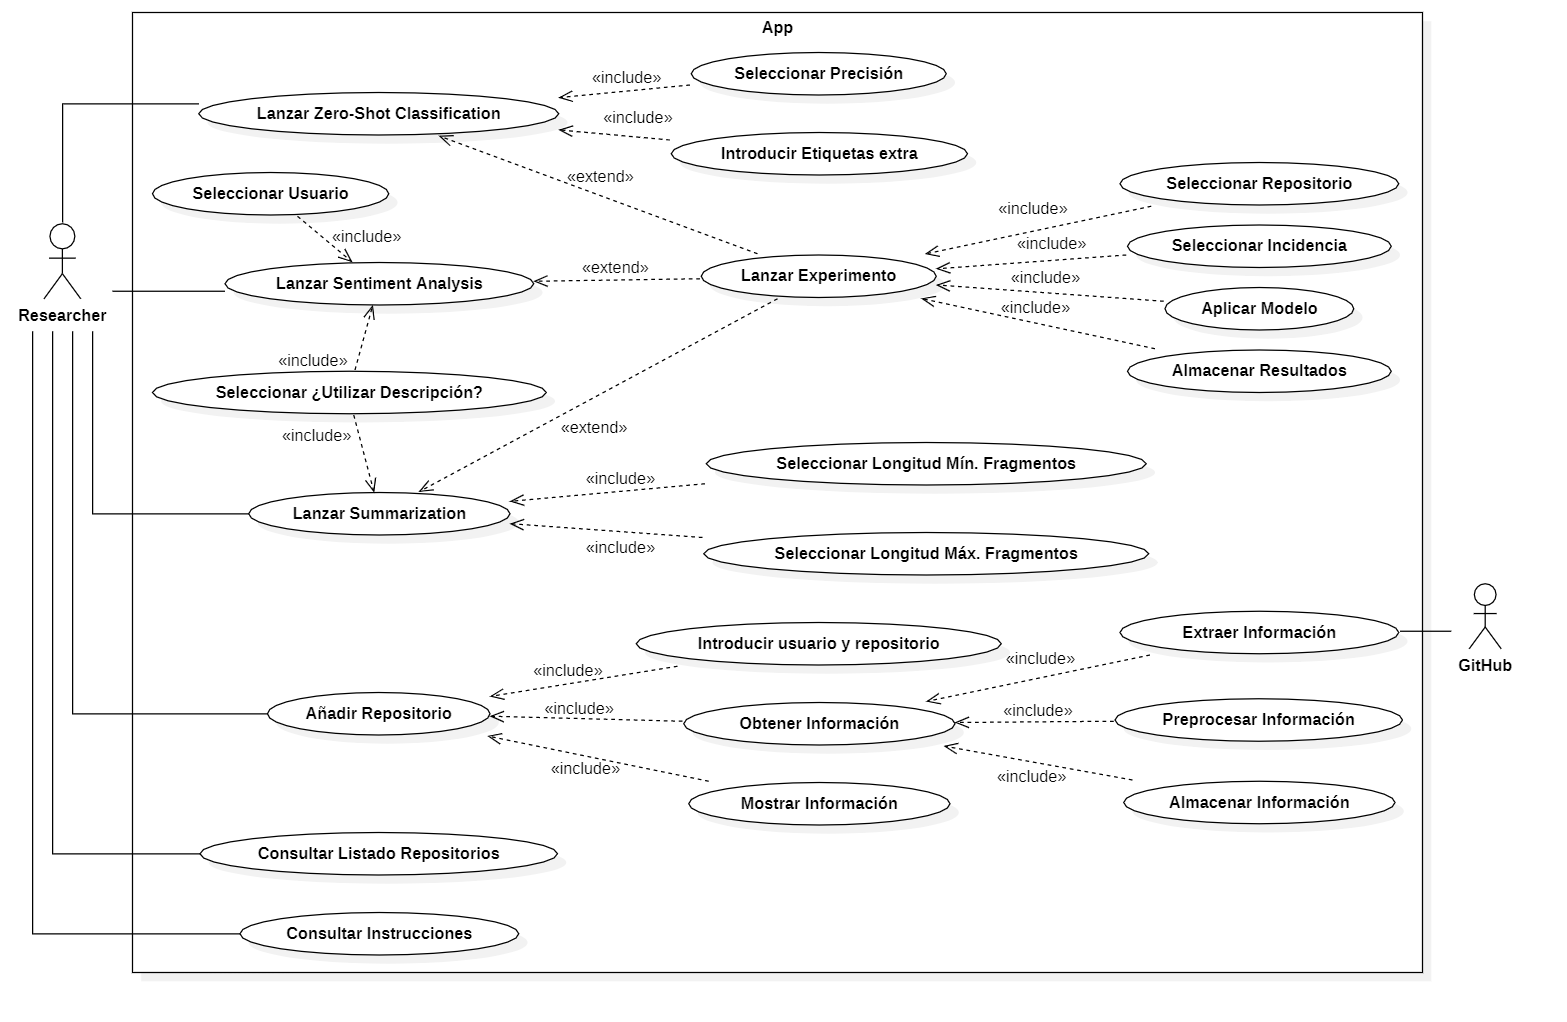
\includegraphics[width=\textwidth]{img/use_case_diagram.png}
	\caption{Diagrama general de casos de uso.}
	\label{fig:use_case_diagram}
\end{sidewaysfigure}